% psyplot chapter

\Chapter{Psyplot}{A flexible framework for interactive data analysis}

\label{chp:psyplot}

\begin{refsection}

%----------------------------------------------------------------------------------------
%	SECTION 1
%----------------------------------------------------------------------------------------

\section{Summary}  \label{sec:psyplot-joss}

\blockquote{
	\textit{From}
	\bibforkey{Sommer2017}
}

\noindent psyplot \citep{Sommer2017} is a cross-platform open source python project that mainly combines the plotting utilities of matplotlib \citep{Hunter2007} and the data management of the xarray \citep{HoyerHamman2017} package and integrates them into a software that can be used via command-line and via a \glsfirst{gui}.

The main purpose is to have a framework that allows a fast, attractive, flexible, easily applicable, easily reproducible and especially an interactive visualization of data.
 
The ultimate goal is to help scientists in their daily work by providing a flexible visualization tool that can be enhanced by their own visualization scripts.

The framework is extended by multiple plugins: psy-simple \citep{Sommer2017b} for simple visualization tasks, psy-maps \citep{Sommer2017c} for georeferenced data visualization and psy-reg \citep{Sommer2017d} for the visualization of fits. It is furthermore extended by the optional graphical user interface psyplot-gui \citep{Sommer2017e}.


\section{Introduction}  \label{sec:psyplot-review}

The mathematical and statistical processing of climate data is closely related to its visualization and analysis. But in traditional visual analytics literature, these two aspects are commonly treated in separate manners. \cite{KeimAndrienkoFeketeEtAl2008} for instance, (following \cite{Wijk2005}) distinguish two steps of visual analytics, the initial data processing with statistical or mathematical techniques, and a \textit{sense-making loop} of visualization, exploration and the gain of new knowledge. \cite{BoettingerRoeber2019} distinguish the \textit{filtering} step (data processing), and \textit{mapping}/\textit{rendering} step that describes the visualization. Also in the literature there is a clear division between the climate visualization (or visual analytic) papers and the standard statistical or climate literature that describes new methods for data processing. Visualization research focuses mainly on advanced visualization tools such as ParaView \citep{Ayachit2015}, VAPOR \citep{ClyneMininniNortonEtAl2007} or Avizo\footnote{\url{https://www.fei.com/
software/avizo3d/}} \citep[e.g.][]{RautenhausBoettingerSiemenEtAl2018, NockeBuschmannDongesEtAl2015, WongShenLeungEtAl2014, BoettingerRoeber2019} whereas statistical or climate literature commonly uses R \citep{RCT2019}, Python \citep{Oliphant2006, PerezGrangerHunter2011}, \glspl{cdo} \citep{Schulzweida2019} or other command-line tools.

This separation, however, devalues the interplay between the new knowledge from the visualization step, that commonly raises the need for more statistical and mathematical processing of the initial data. This calls for integrated and flexible tools that tackle both steps: the data processing and the visualization, a requirement that is currently not fulfilled by the visualization tools described above. An example software that integrates data processing and data visualization is provided with the Earth System Model Evaluation Tool (ESMValTool) \citep{EyringRighiLauerEtAl2016}. This framework provides common diagnostics for \glspl{esm} to enable model intercomparisons. The tool, however, has limited interactivity and a slow learning curve for the implementation of new diagnostics.

This lack leads to large efforts of climate scientists to develop scripts for the data processing and visualization. They usually do not follow a systematic framework and as such need to be adapted every time a new project starts which also make them difficult to share with other researchers. The new \textit{psyplot} framework wants to generalize this data processing and visualization by providing a framework that is highly flexible, interoperates with standard computational data processing tools and enables flexible visualizations and adaptations. The software is written in the programming language Python \citep{PerezGrangerHunter2011} and builds upon the visualization package \textit{matplotlib} \citep{Hunter2007} and the N-dimensional array processing package \textit{xarray} \citep{HoyerHamman2017}, that closely interoperates with the numeric packages numpy and scipy \citep{JonesOliphantPetersonEtAl2001, Oliphant2006} and the parallel computing library dask \citep{DDT2016}. Due to the flexibility of Python, it can be used from the command-line, a \gls{gui} (section \ref{sec:psyplot-gui}) or jupyter notebooks\footnote{\url{https://jupyter.org/}} \citep{KluyverRaganKelleyPerezEtAl2016}. As such, it supports out-of-core computation (i.e. the processing of data too large to fit into memory), a rich set of visualization methods from matplotlib, and can be extended to other visualization packages, such as the 3D-visualization framework VTK \citep{Sommer2019a}.

The next section \ref{sec:psyplot-framework} provide an overview of the framework with its data model, plugins and \gls{gui}. Sections \ref{sec:psyplot-conclusions} and \ref{sec:psyplot-outlook} finally discuss further usage and extensions to the software. For more information, usage and implementation examples I also refer to the online documentation \url{https://psyplot.readthedocs.io}.

\section{The psyplot framework}  \label{sec:psyplot-framework}

The psyplot framework consists of three parts: The core structure that is built upon \textit{xarray} and provides the general infrastructure (section \ref{sec:psyplot-model}), the plugins that use the plotting functionalities of \textit{matplotlib} (section \ref{sec:psyplot-plugins}), and the \gls{gui} (section \ref{sec:psyplot-gui}).


\subsection{Data model}  \label{sec:psyplot-model}

\subsubsection{Psyplot and xarray}  \label{sec:psyplot-dependencies}

psyplot acts as a high-level interface into the packages \textit{xarray} and \textit{matplotlib}. The first one is a recent package for N-dimensional labeled arrays that adopts Unidata’s self-describing Common Data Model on which the network Common Data Form (netCDF) is built \citep{RewDavis1990, BrownFolkGoucherEtAl1993, HoyerHamman2017}. The package integrates with standard python from the python environment, such as the computing and analysis packages numpy \citep{Oliphant2006}, scipy \citep{JonesOliphantPetersonEtAl2001, Oliphant2007}, pandas \citep{McKinney2010} and statsmodels \citep{SeaboldPerktold2010}, but also offers intuitive interfaces for other packages, such as a package for empirical orthogonal functions \citep[EOFs, ][]{Dawson2016}, \glspl{cdo} \citep{Mueller2019}, fourier transforms \citep{UchidaRokemNicholasEtAl2019} and many more\footnote{\label{foot:xraccessors} several packages related to xarray are listed in the docs at \url{http://xarray.pydata.org/en/stable/related-projects.html} and psyplots integration (accessors) in particular is shown at \url{https://psyplot.readthedocs.io/en/latest/accessors.html}.}. This large potential for extension distinguishes psyplot from other high-level visualization software, such as ParaView or Vapor, as such python packages can be implemented as a so-called \textit{formatoption} (without hyphen, see below) or used in a pre-processing step.

\subsubsection{Psyplot core structure}  \label{sec:psyplot-core}  

\begin{figure}
	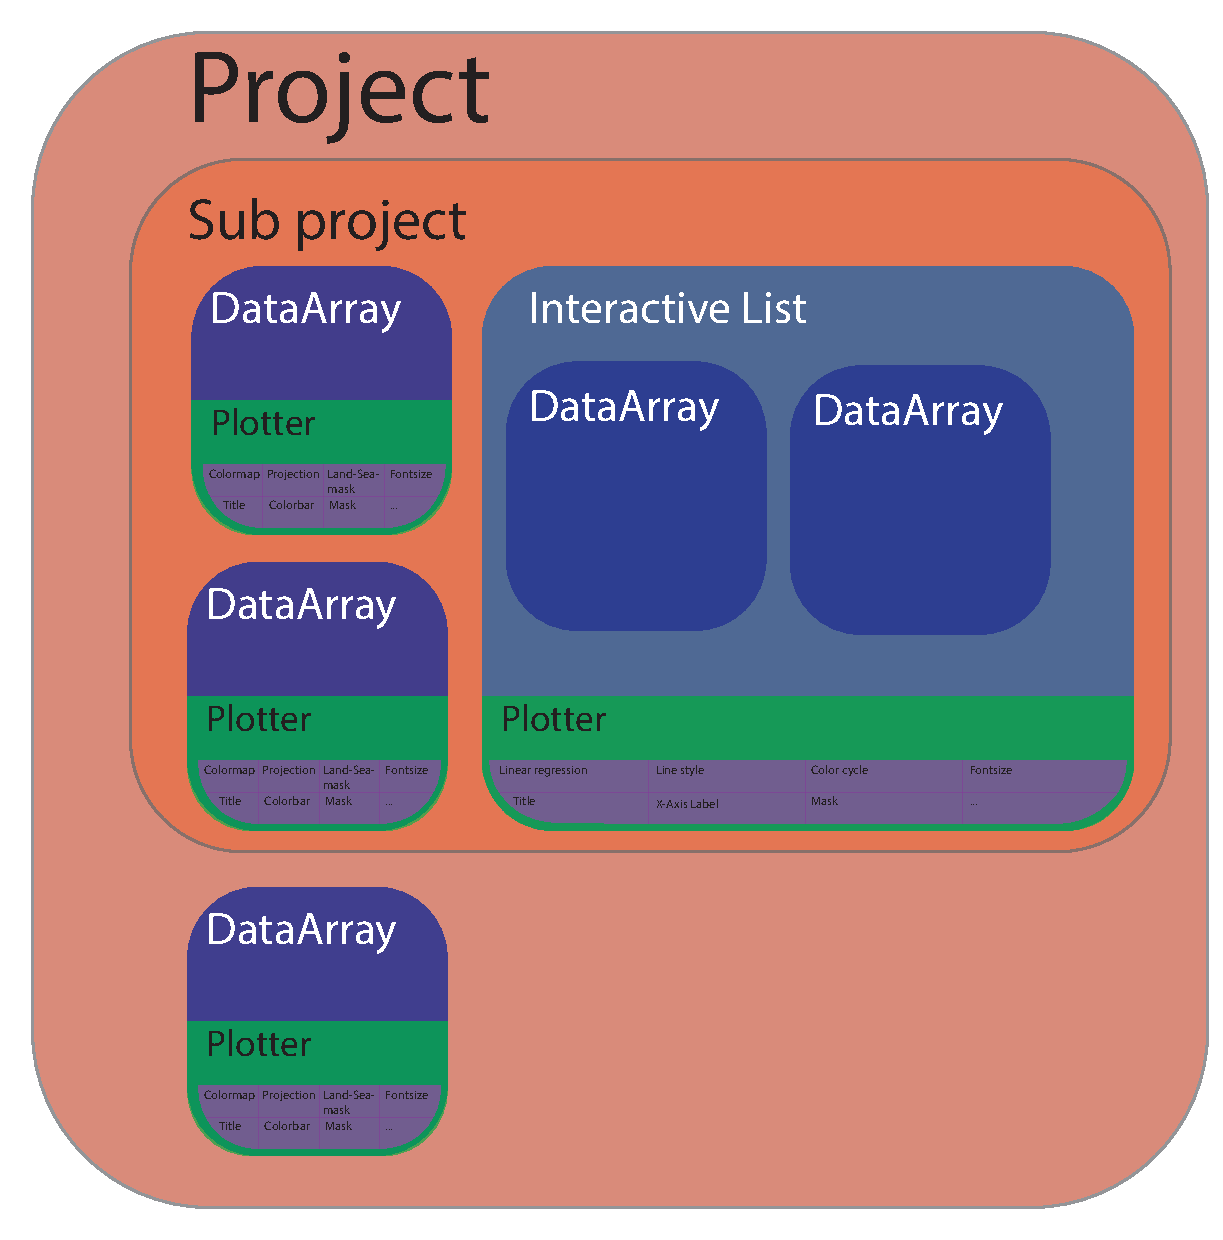
\includegraphics[width=\linewidth]{psyplot-figures/psyplot_framework.pdf}
	\caption[The psyplot core framework]{The psyplot core framework. A (sub) project consists of n-dimensional data arrays or a list of these that are each visualized by a plotter. Each plotter consists of a set of \textit{formatoptions} that control the appearance of the plot or performs data manipulation.}
	\label{fig:psyplot-core}
\end{figure}

The core structure of psyplot consists of five base classes that interact with each other, the visualization objects \textit{Plotter} and its \textit{Formatoptions}, the data objects \textit{DataArray}, an \textit{InteractiveList} of them, and a collection of all of them, the psyplot \textit{Project}. It is schematically visualized in figure \ref{fig:psyplot-core}.

The most high-level \gls{api} object is the psyplot project that consists of multiple data objects that are (or are not) visualized. The main purpose is a parallel handling of multiple plots/arrays that may also interact with each other (e.g. through the sharing of \textit{formatoptions}). It mainly spreads update commands to its contained objects, but also serves as a filter for the data objects. Furthermore, one project may be split up into sub projects which then only control a specific part of the main project, e.g. for a specific formatting of only a small part of the data.

The next level is the \textit{DataArray} from the xarray package (or more explicitly, its accessor, the \textit{InteractiveArray}$^{\ref{foot:xraccessors}}$), that holds the data of one (or more) variables (e.g. temperature) and its corresponding coordinates (e.g. time, latitude, longitude, etc.). It may be one or multidimensional depending on the chosen visualization method. psyplot offers several methods to provide the coordinates for the plotting of different grids to make the visualization easier. The software can interpret CF Conventions\footnote{\url{http://cfconventions.org}} and UGRID conventions for unstructured grids \citep{JagersStuebeGrossEtAl2018}.

Multiple of these arrays can also be grouped together into an \textit{InteractiveList} that shall be visualized by the same plot method (e.g. multiple lines or a scalar field with overlying vector field).

The visualization part in the framework is managed by the \textit{Plotter} class, a collection of multiple \textit{Formatoptions}. Each plotter subclass is designed to visualize the data in a specific manner (e.g. via line plots, violin plots, or map plots) and is completely defined through it’s \textit{formatoptions}.

\textit{Formatoptions} are the core of the psyplot structure. The standard functionality of a formatoption is to control the visual appearance of one aspect of the plot (e.g. through the colormap, figure title, etc.). It is, however, completely unlimited and can also do data manipulations or calculations. The psy-reg plugin for example (see section \ref{sec:psyplot-plugins}) implements a formatoption that performs a regression through the data that is then visualized. As mentioned earlier, each plotter is set up through its \textit{formatoptions} where each formatoption has a unique formatoption key inside the plotter. This formatoption key (e.g. \textit{title} or \textit{cmap}) is what is used for updating the plot, manipulating the data, etc.. \textit{Formatoptions} might also interact with other \textit{formatoptions} inside the plotter or from other plotters. This concept of \textit{formatoptions} allows to use the same formatoption with all different kinds of plotters and the interaction of multiple plots with each other. Common plot features, such as the figure title, colormap, etc., therefore do not have to be implemented explicitly for every plotter but can be used from existing implementations. This framework also allows a very easy integration and development of own \textit{formatoptions} with a low or high level of complexity.

\subsection{Psyplot plugins}  \label{sec:psyplot-plugins}

The psyplot package provides the core of the data management described in the previous section \ref{sec:psyplot-model}. The real visualization is implemented in external plugins. The advantage of this approach is an increased flexibility of the entire framework (collaborations can evolve through dedicated plugins) and of managing the various dependencies of the packages. As such, the dependencies of psyplot are rather week (only xarray is needed), but the dependencies of the plugins can be more extensive (e.g. for geo-referencing or advanced statistics). 

Each plugin defines new \textit{Plotters} and \textit{Formatoptions} that are specific to the purpose of the visualization/analysis task. The plotters can also be implemented as a plot method (see supplements \ref{sec:psy-simple-plotmethods} to \ref{sec:psy-strat-plotmethods}) and accessed through the psyplot core \gls{api} (see supplements \ref{sec:psyplot-example} for an example).

The current lists of plugins include \textit{psy-simple} for rather simple and standard visualization tasks, \textit{psy-maps} for geo-referenced plots, \textit{psy-reg} for statistical analysis visualization, and \textit{psy-strat} for stratigraphic diagrams.

\subsubsection{psy-simple: The psyplot plugin for simple visualizations}

Much of the functionality that is used by other plugins is developed in the psy-simple plugin. This package targets simple visualizations and currently includes plot methods for one-dimensional data: line plots, bar plots and violin plots; for two-dimensional data: scalar plots, vector plots and combined scalar and vector plots; and plots that do not require complex data manipulation: a density plot and a plot of the weighted geographic mean. A full list of examples is provided in the supplementary material, section \ref{sec:psy-simple-plotmethods}.

This package also implements most of the functionality to handle unstructured grids in 2D visualizations and defines most of the commonly used \textit{formatoptions}. The latter include text manipulation (such as plot title, figure title, x- and y-axis labels, etc.), data masking, x- and y-axis tick labeling and positioning, as well as color coding for 2D plots (colormap, colormap sections, etc.).

\subsubsection{psy-maps: The psyplot plugin for visualizations on a map}

psy-maps builds on top of the psy-simple plugin and extends its functionality for visualizations on a map using the functionalities of the cartopy package \citep{Cartopy} (see supplements \ref{sec:psy-maps-plotmethods} for examples). It simplifies as such the automated generation of maps for climate model data through the flexibility of the psyplot framework.

psy-maps currently implements additional \textit{formatoptions} for choosing the projection of the map, selecting the geographic region, drawing the contintens or shaded reliefs of land and ocean, and more. One feature that distinguishes psy-maps from other visualization software, even from pure cartopy, is the ability to visualize unstructured geo-referenced grids on the map. For this purpose, triangles are projected in a pre-processing step to the target projection, prior to the visualization with matplotlib. This drastically increases the performance and makes it possible to visualize even very large data sets. As such, psy-maps visualizes a global scalar field on a hexagonal grid of roughly 4.4 million grid cells ($\approx 13$ km resolution) in roughly 3.5 minutes. The interactive usage of such a large dataset is however limited by the functionalities of matplotlib to handle such an immense amount of data.

\subsubsection{psy-reg: The psyplot plugin for visualizing and calculating regression plots}

psy-reg performs regression analysis on 1D variables using the methods of the stats-models \citep{SeaboldPerktold2010} and scipy \citep{JonesOliphantPetersonEtAl2001, Oliphant2007} packages, and visualizes the results with the functionalities of the psy-simple plugin. As such, it implements \textit{formatoptions} for univariate regressions, confidence intervals via bootstrapping, and combined plots of the data density and the fitted model (see also supplements \ref{sec:psy-reg-plotmethods}). The necessity for this package arose from the need to visualize a regression model, compare it (visually) with the original data and to use it afterwards. Other python packages either focus only on the generation of the regressions (such as statsmodels or scipy), or on their visualization (such as seaborn \citep{WaskomBotvinnikOKaneEtAl2018}). The psyplot plugin makes it possible to generate the visualization and to access the underlying regression model parameters and uncertainties.

psy-reg has been heavily used for the parameterization of the weather generator in chapter \ref{chp:gwgen} which also gave the initial motivation for the package. 

\subsubsection{psy-strat: A psyplot plugin for stratigraphic plots}

psy-strat \citep{Sommer2019} is the latest plugin for psyplot that has been developed for stratigraphic diagram visualization. It is particularly designed for the straditize software \citep[chapter \ref{chp:straditize}]{SommerRechChevalierEtAl2019} and was motivated by the need for an automated creation of pollen diagrams. One example of such a diagram is provided in the supplementary material, section \ref{sec:psy-strat-plotmethods}.

As the psy-reg and psy-maps plugins, psy-strat uses the functionalities of the psy-simple plugin for a visualization of multiple variables in separate diagrams that share one common vertical axis (usually age or depth)\footnote{See \href{https://psy-strat.readthedocs.io}{psy-strat.readthedocs.io} for an example of psy-strat.}. Additionally, besides the integration that is common for every psyplot plugin (see next section \ref{sec:psyplot-gui}), psy-strat contains additional functionalities for the psyplot \gls{gui}. This implementation allows the user to select and reorder the variables (pollen taxa) that are shown in the stratigraphic diagram.


\subsection{The psyplot Graphical User Interface}  \label{sec:psyplot-gui}

\begin{figure}
	\begin{tikzpicture}
		\node[anchor=south west,  inner sep=0] (image) at (0,0,0) {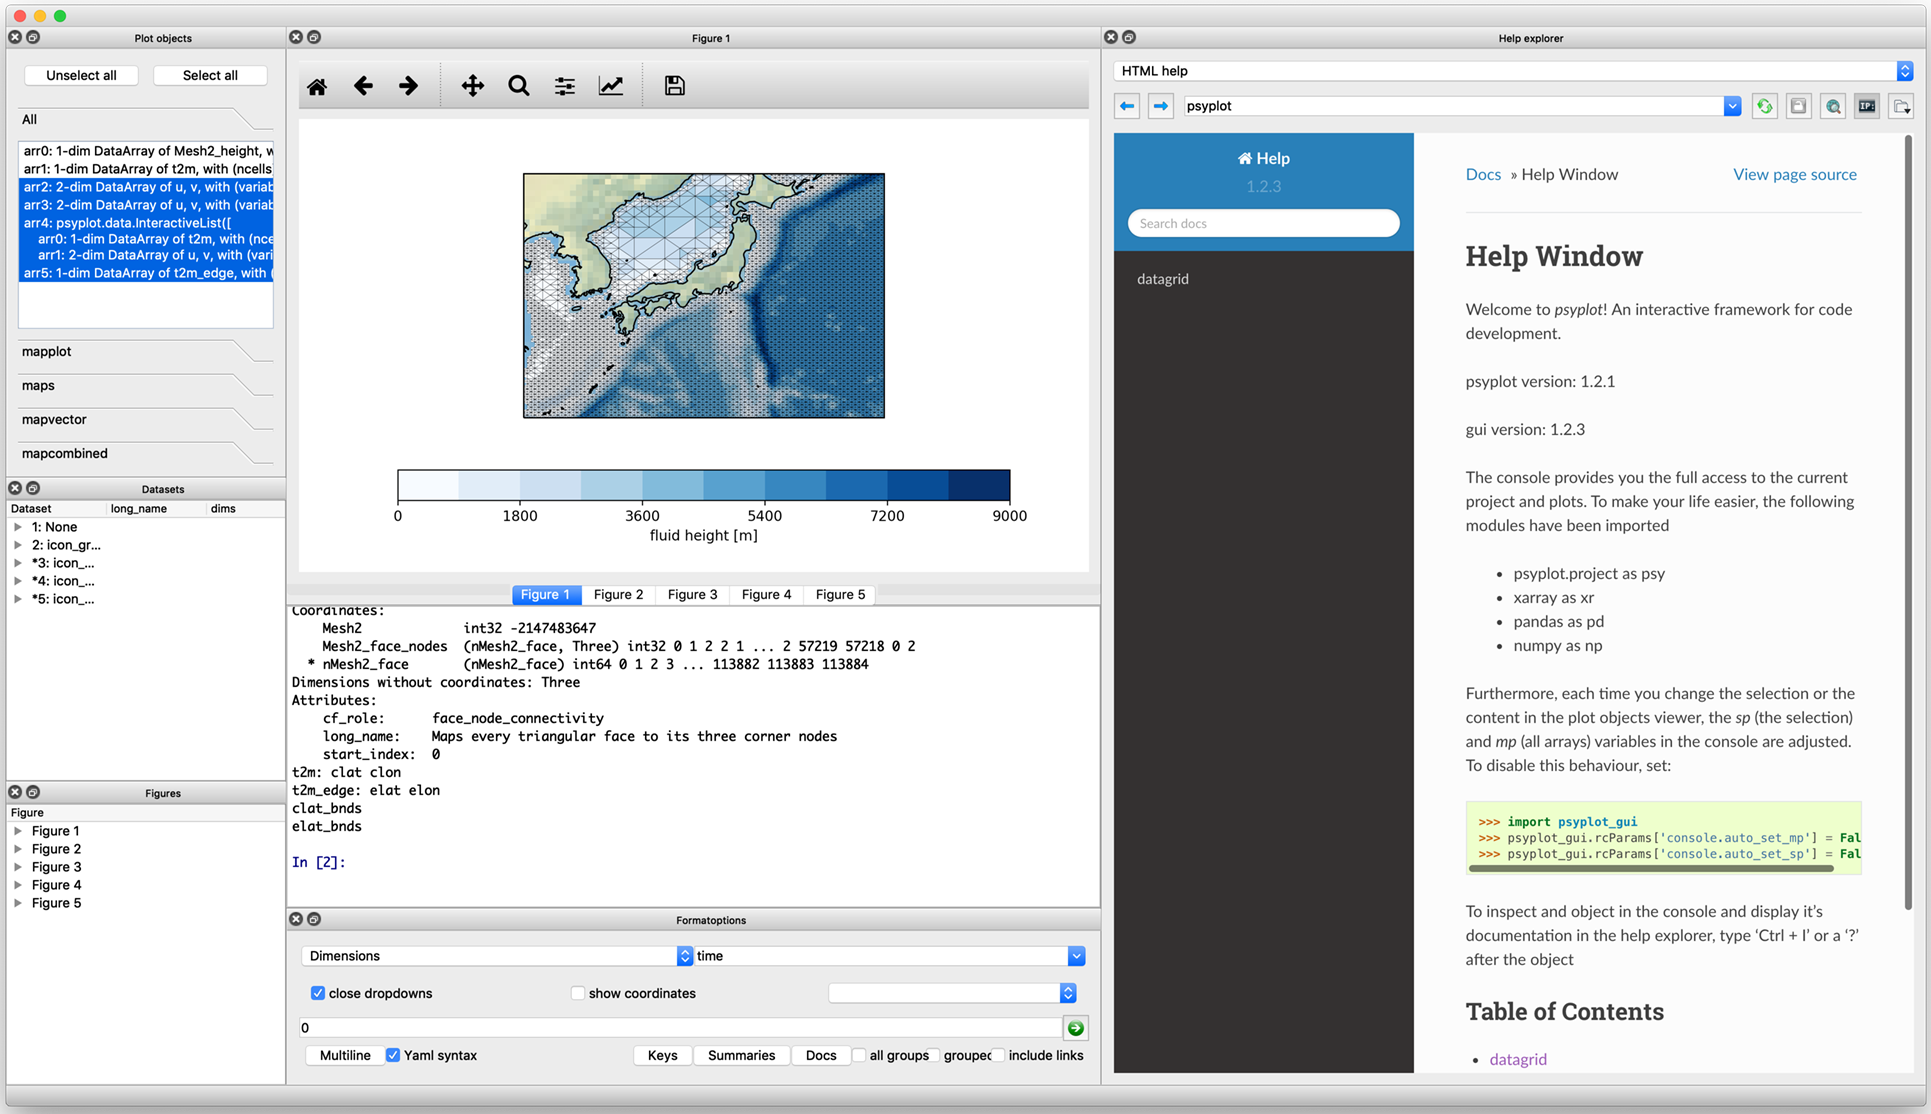
\includegraphics[width=\linewidth]{psyplot-figures/psyplot-gui.png}};
		\node[] (figures) [above=of image, xshift=-0.1\linewidth, yshift=-0.5cm, fill=red!50] {Figures};
		\node (project) [left=of figures, xshift=-0.1\linewidth, fill=red!50] {Project content};
		\node (help) [right=of figures, xshift=0.2\linewidth, fill=red!50] {Help explorer};
		\node (formatoptions) [below=of image, xshift=-0.1\linewidth, yshift=0.5cm, fill=red!50] {Formatoptions};
		\node (console) [above=of formatoptions, yshift=1.5cm, fill=red!50] {Console};
	\end{tikzpicture}
%	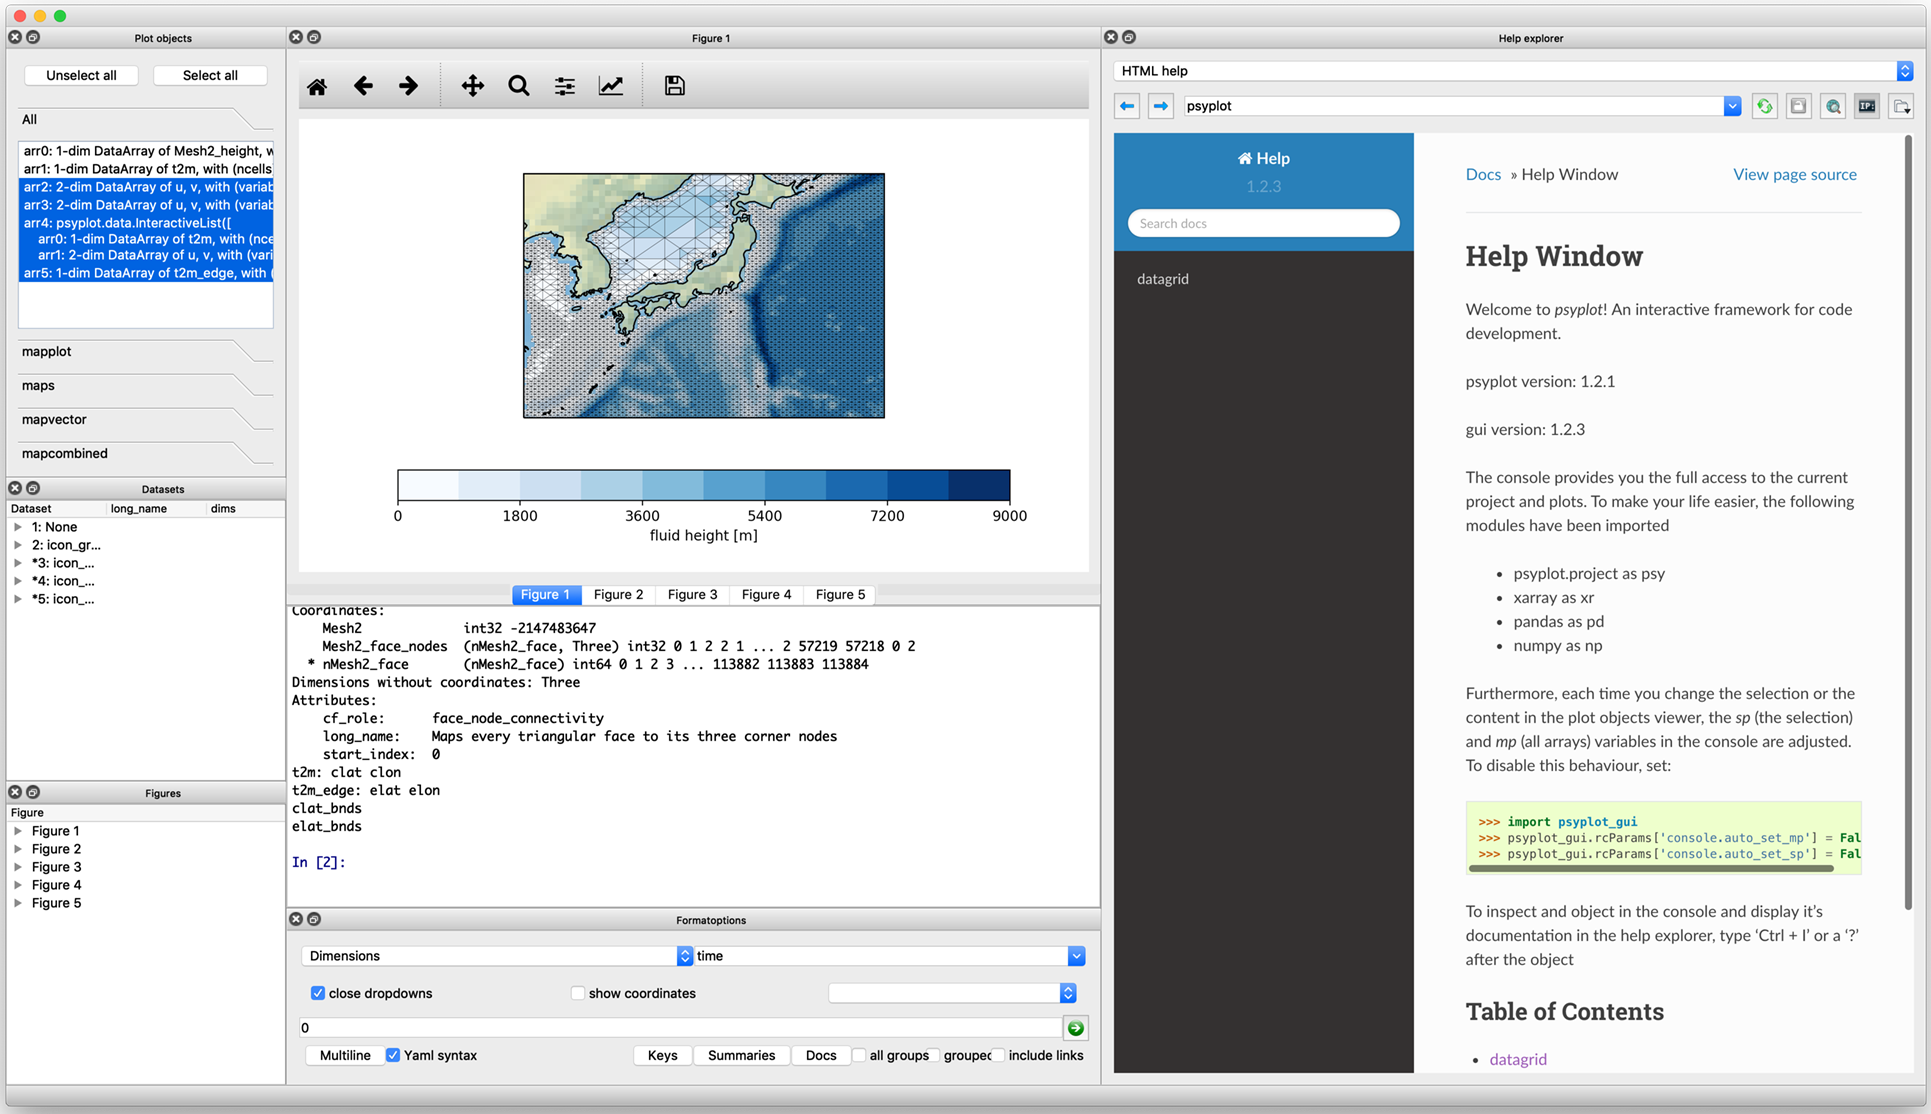
\includegraphics[width=\linewidth]{psyplot-figures/psyplot-gui.png}
	\caption[Screenshot of the psyplot GUI]{Screenshot of the psyplot \gls{gui}. The left part shows the content of the psyplot project, the upper center the plots, and the right part contains the help explorer. Below the plots, there is also the IPython console for the usage from the command line and a widget to update the \textit{formatoptions} of the current project.}
	\label{fig:psyplot-gui}
\end{figure}

\begin{figure}
	\centering
	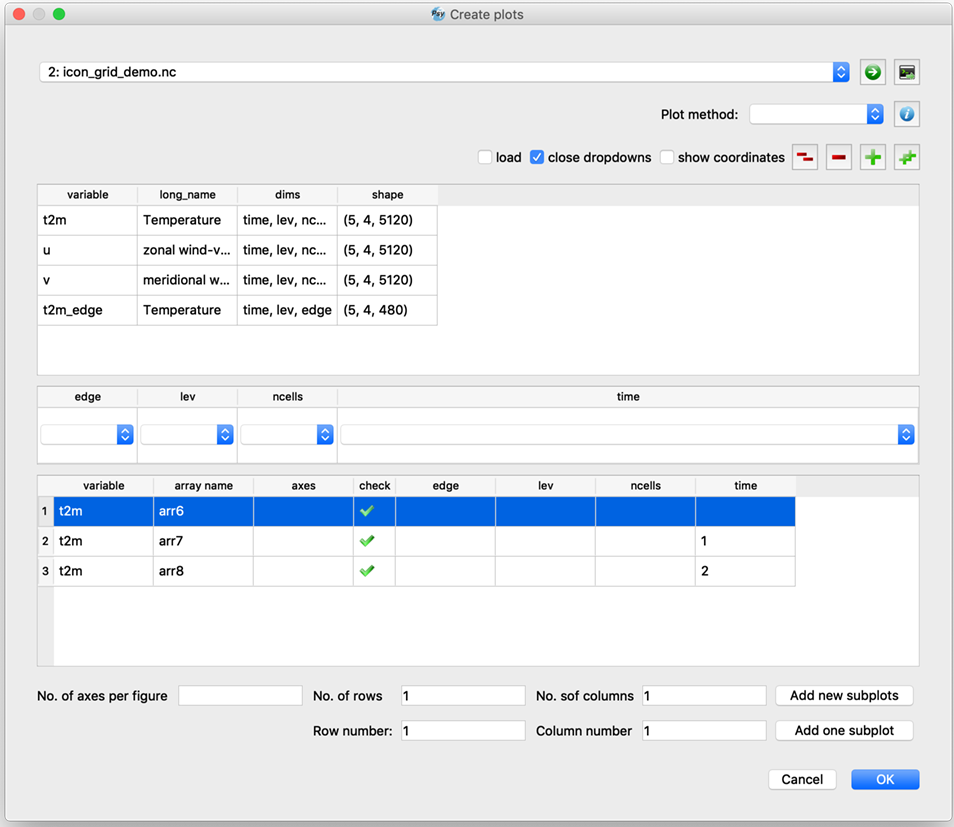
\includegraphics[width=0.7\linewidth]{psyplot-figures/plot-creator.png}
	\caption[psyplot Gui plot creation dialog]{Plot creation dialog to generate new figures from an xarray dataset.}
	\label{fig:psyplot-gui-plot-creator}
\end{figure}

Psyplots objective of providing a platform for flexible and convenient data analysis is further approached with the \textit{psyplot-gui} package. This extension to the framwork provides a \gls{gui} for simplified access to the plotting features in psyplot.

A strong focus of this interface is, again, the flexibility. psyplot-gui is based on the cross-platform PyQt5 library\footnote{PyQt5 can be accessed via \url{https://riverbankcomputing.com/software/pyqt/intro}.}, a very flexible and frequently used package for \acrlongpl{gui}. This enables other software to develop additional features for the package (see psy-strat in the previous section \ref{sec:psyplot-plugins}, for instance, or straditize in chapter \ref{chp:straditize}) and to flexibly change the layout of the application. The \gls{gui} is complemented with an interactive console to provide a fully integrated python environment for data analysis.

The next paragraphs provide an overview on the various widgets, that are also displayed in figure \ref{fig:psyplot-gui} and \ref{fig:psyplot-gui-plot-creator}. 

\subsubsection{Console}
The central aspects to guarantee flexibility of the application is an in-process IPython console, based on the qtconsole package\footnote{\url{https://github.com/jupyter/qtconsole}} that provides the possibility to communicate with the psyplot package via the command line and to load any other module or to run any other script or notebook, or even to run commands in different programming languages, such as R \citep{RCT2019} or Julia \citep{BezansonEdelmanKarpinskiEtAl2017}. The console is fully integrated both ways into the \gls{gui}. The documentation of every python object in the terminal, for instance, can be viewed in the help explorer of the GUI. And vice versa: a change of the current project through the project content widgets, also changes the corresponding python variable in the shell. 

\subsubsection{Help explorer}
As a complement to the console, the \gls{gui} contains a help explorer to provide immediate and dynamic access to the documentation of python objects in the console, rendered as an HTML webpage\footnote{The help explorer widget has been originally motivated by the \textit{Help} widget of the Scientific PYthon Development EnviRonment, Spyder (\url{https://www.spyder-ide.org/}) and uses the sphinx package \citep{Hasecke2019} to convert restructured Text into HTML.}. Furthermore, the help explorer is connected to multiple other widgets of the \gls{gui} in order to provide a dynamically generated documentation. The documentation of available \textit{formatoptions} in the psyplot project, for instance, are rendered as HTML upon request, in order to make the various plot methods more accessible. The same principle works for the plot methods that are accessible in the plot creator.

\subsubsection{Plot creator}
The plot creator (figure \ref{fig:psyplot-gui-plot-creator}) is the starting point of the \gls{gui} into the psyplot framework (at least, if one does not use the console or a script to generate the plots). It loads data from the disk or the in-process console, and essentially provides a wrapper around the psyplot plotting call (see suppl. section \ref{sec:psyplot-example}). It additionally displays the documentation of the method and its associated \textit{formatoptions}. This widget creates new plots, that are appended to the psyplot project and are accessible through the console and the project content widgets.

\subsubsection{Project content}
The psyplot project is the most high-level \gls{api} element in the psyplot framework (see section \ref{sec:psyplot-core}) and is displayed in the project content widgets of the \gls{gui}. All other elements, such as the \textit{formatoptions} widget or the plot creator, are interfering with the project, and it is accessible as a variable in the console. The project content widget can be used to see the various items in the project, but it is also used to select the specific items for the so-called \textit{current} sub-project. The latter is dynamically set in the console through the \texttt{sp} variable and it is used by the \textit{formatoptions} widget to update the plotting parameters of the selected items.

\subsubsection{Formatoptions}
As mentioned in section \ref{sec:psyplot-core}, \textit{formatoptions} are the core elements in psyplot that control the figure aesthetics of the plots and/or perform data manipulations. The generic \textit{formatoptions} widget provides access to these parameters, in order to update them for the selected items in the current project. The formatoption itself (i.e. the python object) can in turn generate a widget that is implemented in the \textit{formatoptions} widget, to make the available options more accessible. The \textit{title} formatoption, for instance, generates a drop-down menu to select variable attributes (e.g. variable name, variable units, etc.) which is then embedded in the \textit{formatoptions} widget. The modifications of the \textit{formatoptions} via this widgets, updates the figures of the selected items.

\subsubsection{Figures and plots}
The plots generated by the plotting methods are displayed in dedicated widgets inside the \gls{gui} and can be dynamically adjusted using the \textit{formatoptions} widget or the console. The underlying library of the current implemented psyplot plugins, matplotlib, implements multiple backends to display the data interactively, or to export them as PDF, PNG, etc. The psyplot \gls{gui} has implemented a backend on top of the PyQt5 backend of matplotlib, which embeds the figures in the \gls{gui}. psyplot can, however, work with any backend of matplotlib and does not depend on the specific implementation.

\section{Conclusions}  \label{sec:psyplot-conclusions}
psyplot \citep{Sommer2017} is a new data visualization framework that integrates rich computational and mathematical software into a flexible framework for visualization. It differs from most of the visual analytic software such that it focuses on extensibility in order to flexibly tackle the different types of analysis questions that arise in pioneering research. The design of the high-level API of the framework enables a simple and standardized usage from the command-line, python scripts or jupyter notebooks. A modular plugin framework enables a flexible development of the framework that can potentially go into many different directions. The additional enhancement with a flexible \gls{gui} makes it the only visualization framework that can be handled from the conveniently command-line, and via point-click handling. It also allows to build further desktop applications on top of the existing framework.

The plugins of psyplot currently provide visualization methods that range from simple line plots, to density plots, regression analysis and geo-referenced visualization in two dimensions. The software is currently entirely based on the visualization methods of matplotlib \citep{Hunter2007}, the most established visualization package in the scientific python community. However, the framework itself is agnostic to the underlying visualization method and can, as such, leverage a variety of existing analytical software.

\section{Outlook}  \label{sec:psyplot-outlook}

The possibilities for further development of the psyplot framework are numerous, due to its intrinsic generality. The core of the psyplot framework will, in the future, be extended with a standardized algorithm  for the generation of animations. Psyplot projects already have the functionality of being saved to a file and reloaded, but they will also be exportable as python scripts for a more flexible reusability and adaptability. The update process within a psyplot project (currently every item in the project is updated in parallel) also has potential for improvement by using a single-threaded scheduler approach that better reflects if one formatoption depends on the \textit{formatoptions} of another plotter.

The \gls{gui} has especially high potential for further development, as it still lacks widgets to quickly and intuitively modify the visual appearance of the plots. The only possibility inside the \gls{gui} (besides the console) is to use the \textit{formatoptions} widget whose main focus however is on flexibility, rather than usability and has, as such, limited possibilities for adaptation to specific use cases.

Another focus will be the development of new plot methods inside the psyplot framework. The major aspect will be on the development of 3D visualization methods of geo-referenced data, using recently published software that builds on top of the visualization toolkit VTK \citep{SullivanKaszynski2019, SullivanTrainorGuitton2019}, see \cite{Sommer2019a}. psyplot has the unique potential to generate 3D visualizations conveniently from the command line, a distinguishing feature, compared to other visualization software packages, such as ParaView or Vapor. Further potential enhancements for visualizations can involve standard interactive visual analytic tools, e.g. such that the interactive selection of features in one plot affects the visualization in another plot (so-called brushing and linking).

\clearpage

\begin{subappendices}
	\section*{Supplementary material}
	\section{Example call of a plot method}  \label{sec:psyplot-example}
	
	\begin{Verbatim}[commandchars=\\\{\}]
\PY{c+c1}{\PYZsh{} example call for generating a map}
\PY{k+kn}{import} \PY{n+nn}{psyplot.project} \PY{k+kn}{as} \PY{n+nn}{psy}

\PY{n}{maps} \PY{o}{=} \PY{n}{psy}\PY{o}{.}\PY{n}{plot}\PY{o}{.}\PY{n}{mapplot}\PY{p}{(}
    \PY{l+s+s1}{\PYZsq{}}\PY{l+s+s1}{psy\PYZhy{}maps\PYZhy{}demo.nc}\PY{l+s+s1}{\PYZsq{}}\PY{p}{,}  \PY{c+c1}{\PYZsh{} input file name, can also be data in memory}
    \PY{n}{name}\PY{o}{=}\PY{l+s+s1}{\PYZsq{}}\PY{l+s+s1}{t2m}\PY{l+s+s1}{\PYZsq{}}\PY{p}{,}          \PY{c+c1}{\PYZsh{} variable to plot (can also be multiples}
    \PY{c+c1}{\PYZsh{}\PYZsh{}\PYZsh{} formatoptions}
    \PY{c+c1}{\PYZsh{} colorbar label uses meta attributes of netCDF variable}
    \PY{n}{clabel}\PY{o}{=}\PY{l+s+s1}{\PYZsq{}}\PY{l+s+si}{\PYZpc{}(long\PYZus{}name)s}\PY{l+s+s1}{ [}\PY{l+s+si}{\PYZpc{}(units)s}\PY{l+s+s1}{]}\PY{l+s+s1}{\PYZsq{}}\PY{p}{,}
    \PY{c+c1}{\PYZsh{} select colormap}
    \PY{n}{cmap}\PY{o}{=}\PY{l+s+s1}{\PYZsq{}}\PY{l+s+s1}{RdBu\PYZus{}r}\PY{l+s+s1}{\PYZsq{}}\PY{p}{,}
    \PY{c+c1}{\PYZsh{} focus on a specific lonlatbox given by [lonmin, lonmax, latmin, latmax]}
    \PY{n}{lonlatbox}\PY{o}{=}\PY{p}{[}\PY{l+s+s1}{\PYZsq{}}\PY{l+s+s1}{Europe}\PY{l+s+s1}{\PYZsq{}}\PY{p}{,} \PY{l+s+s1}{\PYZsq{}}\PY{l+s+s1}{Europe}\PY{l+s+s1}{\PYZsq{}}\PY{p}{,} \PY{l+m+mi}{0}\PY{p}{,} \PY{l+s+s1}{\PYZsq{}}\PY{l+s+s1}{Europe}\PY{l+s+s1}{\PYZsq{}}\PY{p}{]}\PY{p}{)}

\PY{n}{maps}\PY{o}{.}\PY{n}{show}\PY{p}{(}\PY{p}{)}
\end{Verbatim}
  % generated with pygmentize -o example_call.text example_call.py
	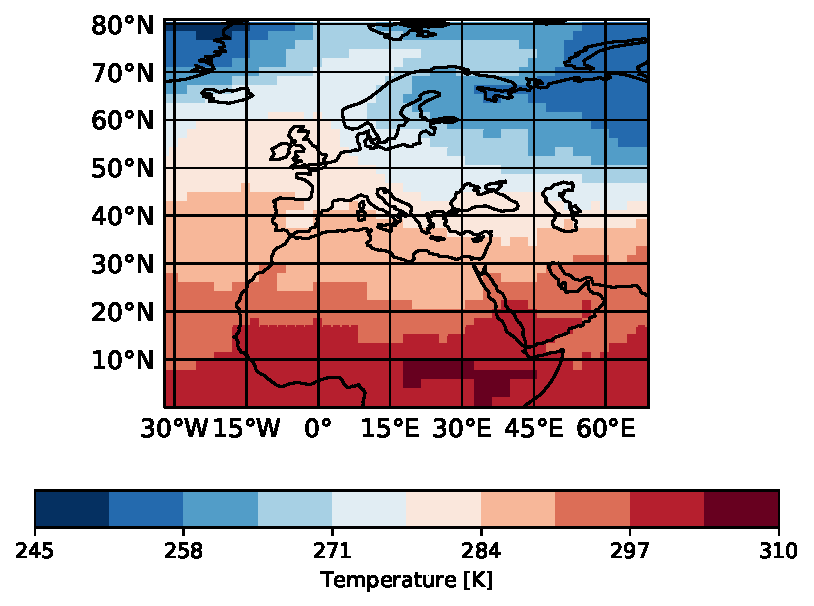
\includegraphics[width=0.45\linewidth]{psyplot-figures/example-call.pdf}
	
	\begin{Verbatim}[commandchars=\\\{\}]
\PY{c+c1}{\PYZsh{} Update the plot, e.g. change projection, plot global}

\PY{n}{maps}\PY{o}{.}\PY{n}{update}\PY{p}{(}\PY{n}{projection}\PY{o}{=}\PY{l+s+s1}{\PYZsq{}}\PY{l+s+s1}{robin}\PY{l+s+s1}{\PYZsq{}}\PY{p}{,} \PY{n}{lonlatbox}\PY{o}{=}\PY{n+nb+bp}{None}\PY{p}{)}
\end{Verbatim}

	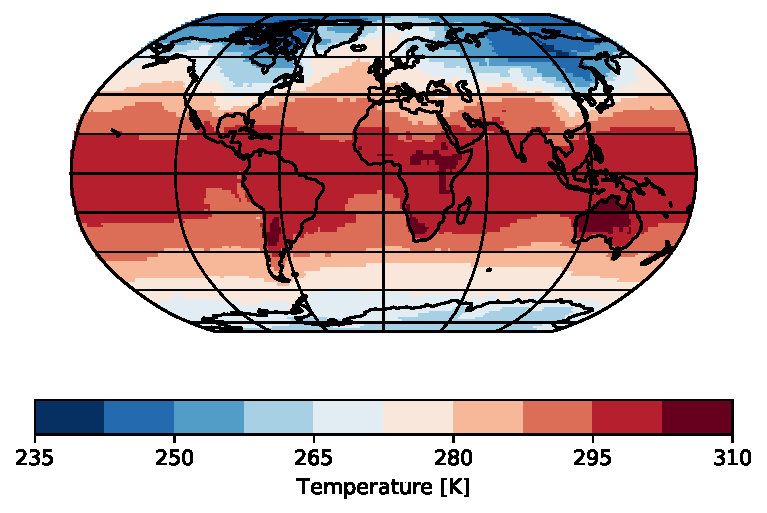
\includegraphics[width=0.6\linewidth]{psyplot-figures/example-update.pdf}
	
	\section{psy-simple plot methods}  \label{sec:psy-simple-plotmethods}
	
		\begin{tabular}[c]{l|p{0.25\linewidth}|p{0.25\linewidth}|p{0.25\linewidth}|}
			\toprule
			\textbf{Plot method} & lineplot & barplot & violinplot \\
			\hline
			\textbf{Example} & 
				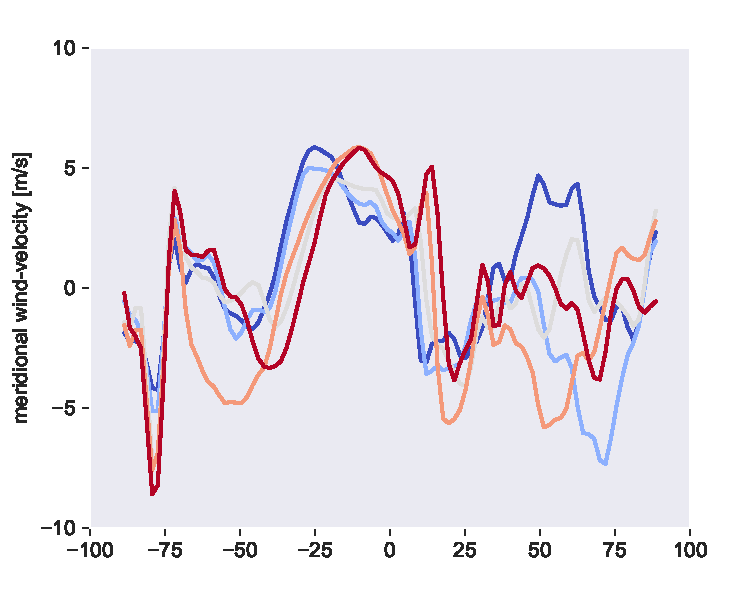
\includegraphics[width=\linewidth, page=1]{psyplot-figures/psy-simple-demo.pdf} &
				\includegraphics[width=\linewidth, page=2]{psyplot-figures/psy-simple-demo.pdf} &
				\includegraphics[width=\linewidth, page=3]{psyplot-figures/psy-simple-demo.pdf} \\
			\midrule
			\midrule
			\textbf{Plot method} & \multicolumn{3}{c}{plot2d} \\
			\hline
			\textbf{Grid type} & rectilinear & \multicolumn{2}{c}{unstructured} \\
			\hline
			\textbf{Example} & 
				\includegraphics[width=\linewidth, page=4]{psyplot-figures/psy-simple-demo.pdf} &
				\includegraphics[width=\linewidth, page=5]{psyplot-figures/psy-simple-demo.pdf} &
				\includegraphics[width=\linewidth, page=6]{psyplot-figures/psy-simple-demo.pdf} \\
			\midrule
			\midrule
			\textbf{Plot method} & \multicolumn{2}{c|}{vector} & combined \\
			\hline
			\textbf{Example} &
				\includegraphics[width=\linewidth, page=7]{psyplot-figures/psy-simple-demo.pdf} &
				\includegraphics[width=\linewidth, page=8]{psyplot-figures/psy-simple-demo.pdf} &
				\includegraphics[width=\linewidth, page=9]{psyplot-figures/psy-simple-demo.pdf} \\
			\midrule
			\midrule
			\textbf{Plot method} & \multicolumn{2}{c|}{density} & {\centering fldmean}  \\
			\hline
			\textbf{Example} & 
				\includegraphics[width=\linewidth, page=10]{psyplot-figures/psy-simple-demo.pdf} & \includegraphics[width=\linewidth, page=11]{psyplot-figures/psy-simple-demo.pdf} & \includegraphics[width=\linewidth, page=12]{psyplot-figures/psy-simple-demo.pdf} \\
			\bottomrule
		\end{tabular}
	

	\section{psy-maps plot methods}  \label{sec:psy-maps-plotmethods}
	
		\begin{tabular}{l|p{0.25\linewidth}|p{0.25\linewidth}|p{0.25\linewidth}|}
			\toprule
			\textbf{Plot method} & \multicolumn{3}{c}{mapplot} \\
			\hline
			\textbf{Grid type} & rectilinear & \multicolumn{2}{c}{unstructured} \\
			\hline
			\textbf{Example} & 
				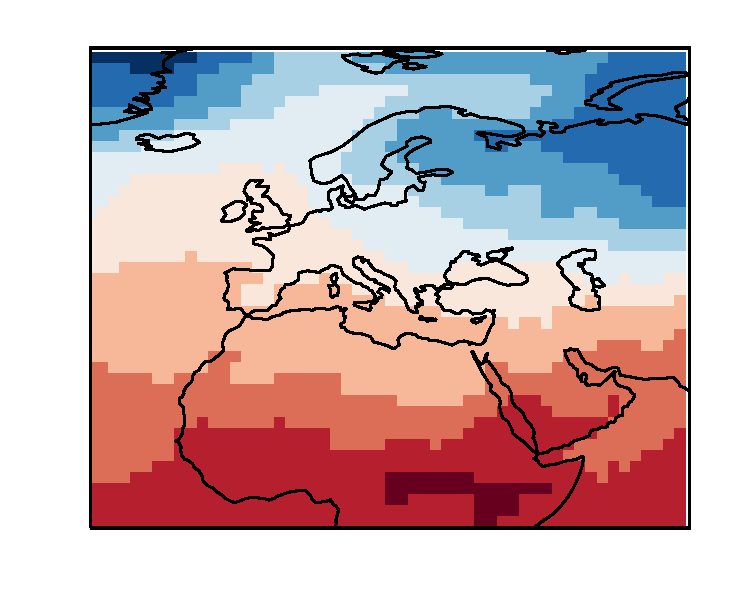
\includegraphics[width=\linewidth, page=1]{psyplot-figures/psy-maps-demo.pdf} &
				\includegraphics[width=\linewidth, page=2]{psyplot-figures/psy-maps-demo.pdf} &
				\includegraphics[width=\linewidth, page=3]{psyplot-figures/psy-maps-demo.pdf} \\
			\midrule
			\midrule
			\textbf{Plot method} & \multicolumn{2}{c|}{mapvector} & combined \\
			\hline
			\textbf{Example} & 
				\includegraphics[width=\linewidth, page=4]{psyplot-figures/psy-maps-demo.pdf} &
				\includegraphics[width=\linewidth, page=5]{psyplot-figures/psy-maps-demo.pdf} &
				\includegraphics[width=\linewidth, page=6]{psyplot-figures/psy-maps-demo.pdf} \\
			\bottomrule
		\end{tabular}
	
	\section{psy-reg plot methods}  \label{sec:psy-reg-plotmethods}
	
		\begin{tabular}{l|p{0.25\linewidth}|p{0.25\linewidth}|}
			\toprule
			\textbf{Plot method} & \multicolumn{2}{c}{linreg} \\
			\hline
			\textbf{Example} & 
				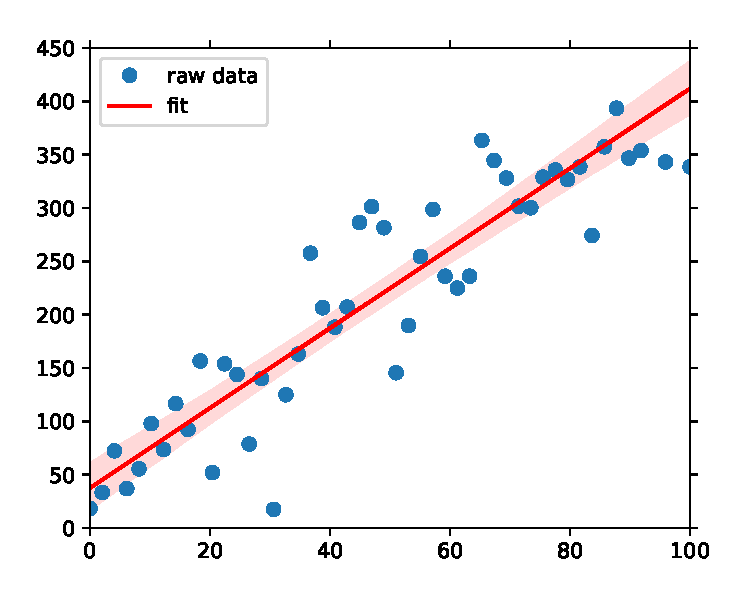
\includegraphics[width=\linewidth, page=1]{psyplot-figures/psy-reg-demo.pdf} &
				\includegraphics[width=\linewidth, page=2]{psyplot-figures/psy-reg-demo.pdf} \\
			\midrule
			\midrule
			\textbf{Plot method} & \multicolumn{2}{c|}{densityreg} \\
			\hline
			\textbf{Example} & 
				\includegraphics[width=\linewidth, page=3]{psyplot-figures/psy-reg-demo.pdf} &
				\includegraphics[width=\linewidth, page=4]{psyplot-figures/psy-reg-demo.pdf} \\
			\bottomrule
		\end{tabular}
	
	\section{psy-strat plot methods}  \label{sec:psy-strat-plotmethods}

		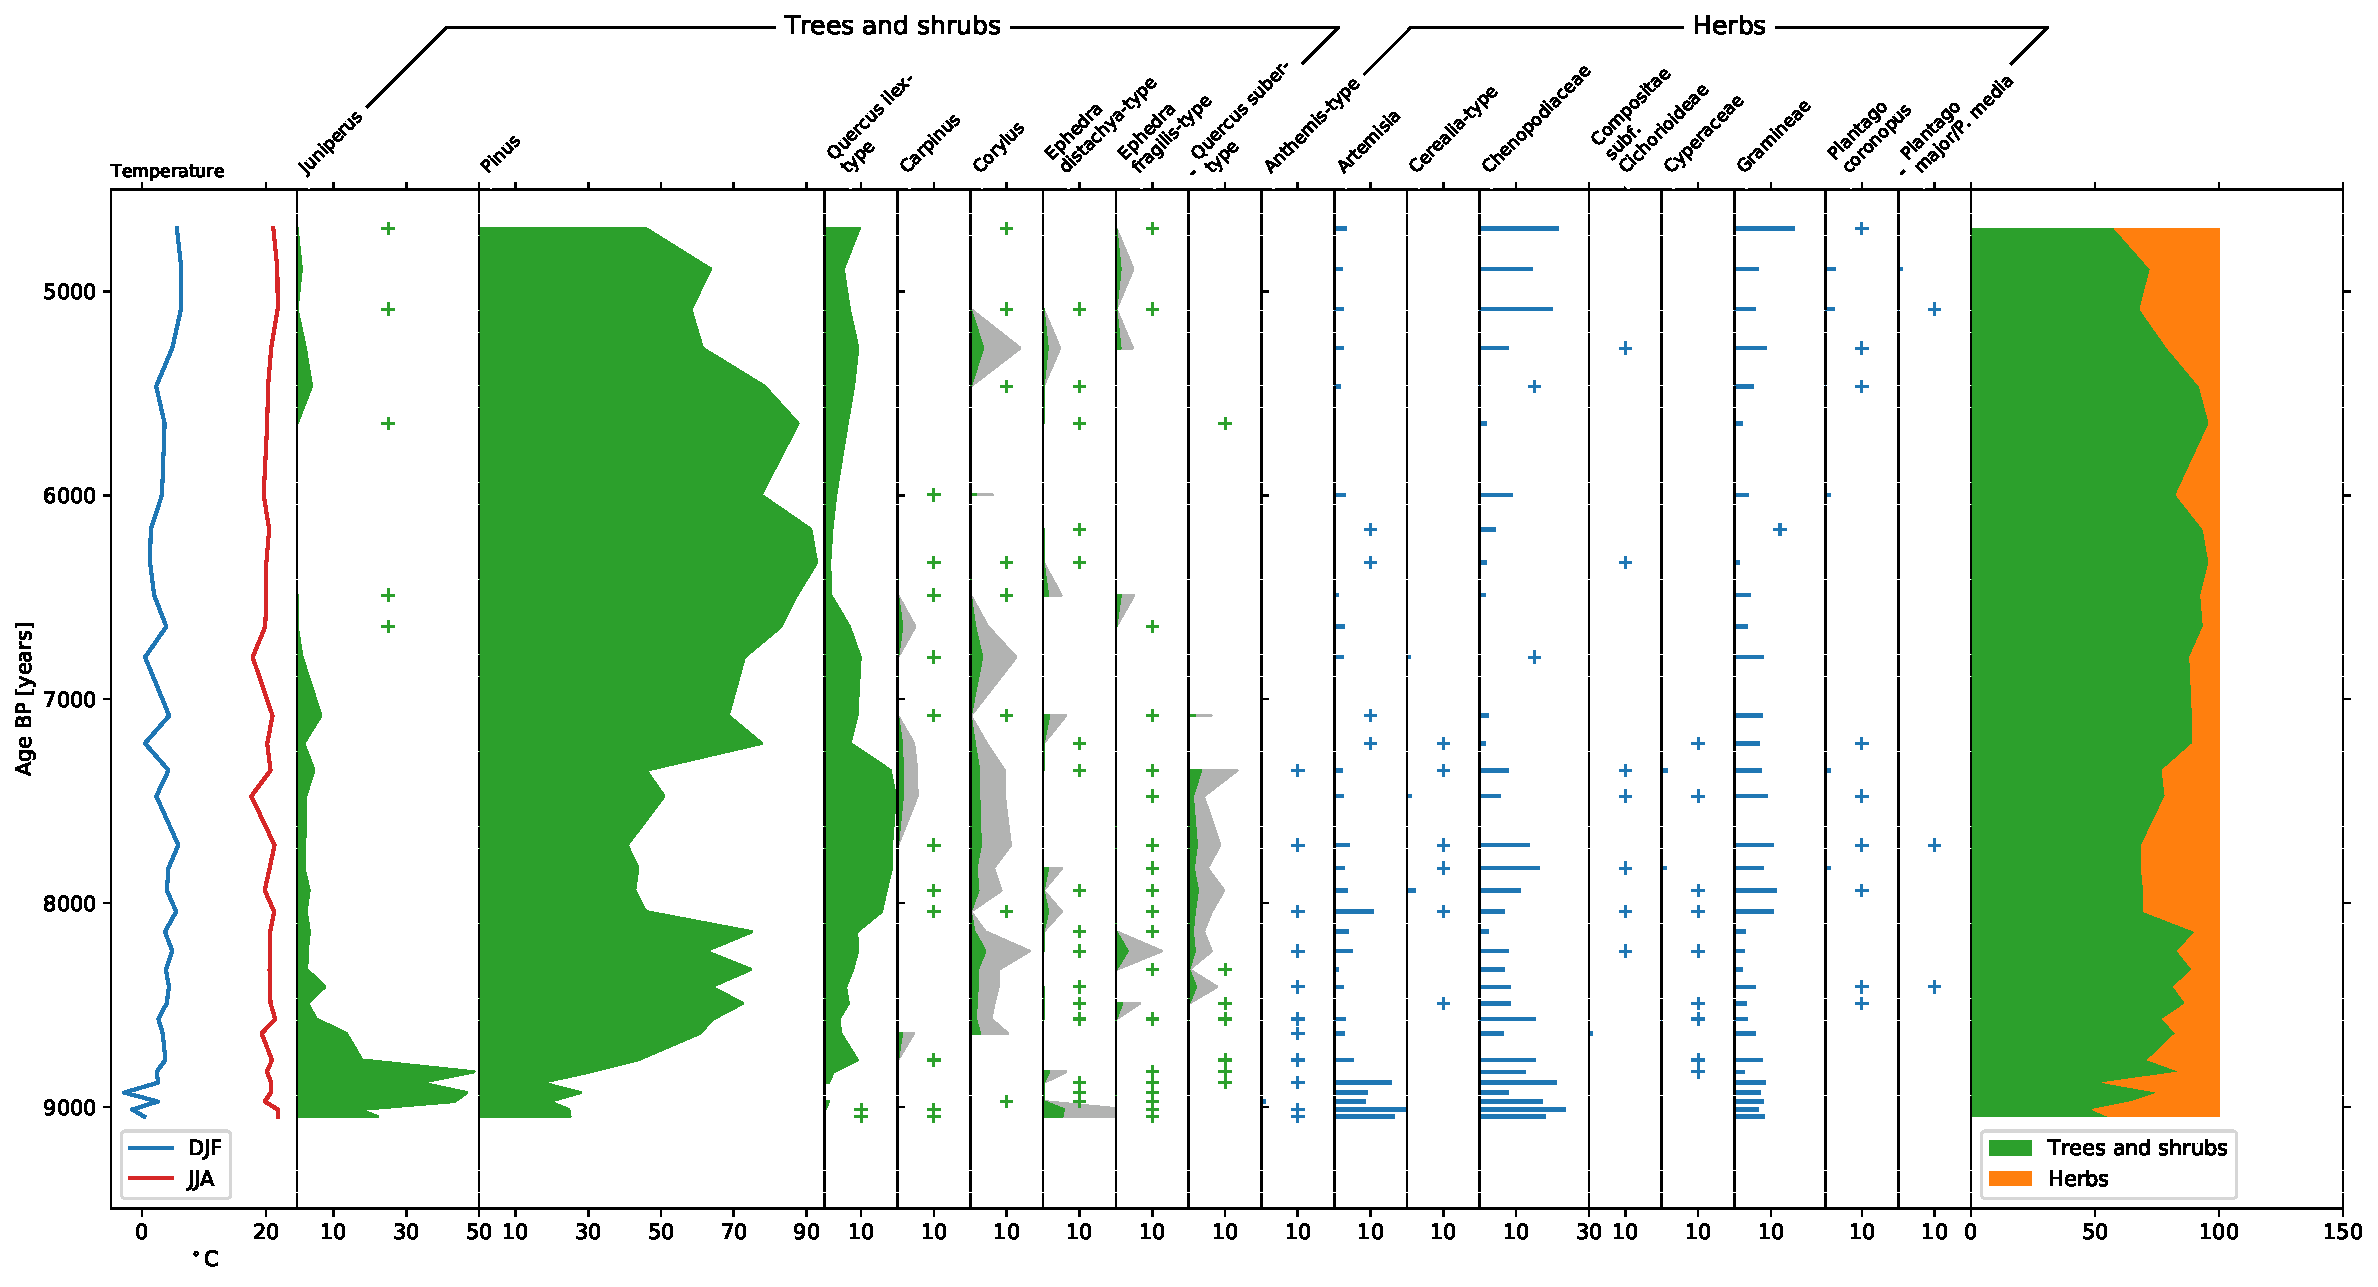
\includegraphics[width=\linewidth]{psyplot-figures/psy-strat-demo.pdf}

\end{subappendices}\

\printbibliography[heading=subbibintoc]

\end{refsection}